\documentclass[12pt,a4paper]{scrartcl}

\usepackage{graphicx}
\usepackage{amsmath}
\usepackage{amsfonts}
\usepackage{amssymb}
\usepackage{bm}
\let\mathbf\bm


\usepackage[T1]{fontenc}
\usepackage[utf8]{inputenc}
\usepackage[magyar]{babel}
\usepackage{lmodern}

\usepackage{placeins}
\usepackage{subcaption}
\usepackage{epstopdf}
\usepackage{xcolor}
\usepackage[hidelinks,unicode]{hyperref}
\hypersetup{
    colorlinks,
    linkcolor={red!50!black},
    citecolor={blue!50!black},
    urlcolor={blue!80!black}
}

\usepackage{cleveref}




\begin{document}
\title{Folytonos közegek mechanikája\\(emelt szint)}
\author{folytkozef17ga, gyakorlat,\\Anyagfizikai Tanszék, Tüzes Dániel}
\maketitle
\tableofcontents
\section*{Kötelező tájékoztatás az első órán}
A \href{https://www.elte.hu/file/ELTE_SZMSZ_II.pdf}{HKR} tartalmazza, hogy mik a feltételei annak, hogy valaki a kurzusra érdemjegyet kapjon, az oktatónak pedig további információkkal kell szolgálnia az első órán.

A \href{http://to.ttk.elte.hu}{Tanulmányi Hivatal oldaláról} elérhető az \href{http://to.ttk.elte.hu/sites/default/files/201819_1_2fev_oktatasihetek_.xls}{oktatási hetek számozása}. Az első gyakorlatot a 2, február 11-ével kezdődő tanulmányi héten kell megtartani.

Amennyiben egy dékáni szünet miatt marad el egy óra, úgy az óra idejében a tantárggyal kapcsolatosan a hallgatók igényei szerint konzultációt tarthatok.

\subsection{Hol és mikor lesznek az órák?}
Pénteken 9:15-10:00 között az északi épület 059-es termében. Összesen 11 tanóra lesz a félévben, ebből 1 a ZH-é, 1 pedig az utolsó heti óra, a dolgozat megbeszéléséé. Az első órát leszámítva így marad 8 óra.

\subsection{Kötelező részvétel}
A gyakorlatokra kötelező bejárni, amelynek célja, hogy a hallgatók az előadáson elhangzott módszereket, elméleti ismeretanyagot saját maguk is konkrét példákon keresztül begyakorolhassák. A gyakorlat megkönnyíti az előadás anyagának megértését és a későbbi vizsgára való felkészülést is. A kurzushoz jelenléti ív tartozik, amely nyilvántartja, hogy a hallgató megjelent-e az órán.

A \href{https://www.elte.hu/file/ELTE_SZMSZ_II.pdf#page=59}{HKR 66.0§-a} rendelkezik, hogy mennyi távollét mellett lehetséges a tárgyra jegyet szerezni. Ezen a tárgyon a HKR szerint lehetséges legrugalmasabb módon eljárva az órák egyharmadát meg nem haladó távollét mellett lehet a tárgyra érdemjegyet kapni.

\subsection{Az órák menete}
A gyakorlaton az előadással kapcsolatos kérdéseket lehet feltenni, valamint speciális eseteket fogunk kézzel kiszámolni, kitűzött házi feladatokat megbeszélni. Ez 8 alkalomra jelent otthoni felkészülést, gyakorlást és házi feladat megoldást is.

\subsection{Kurzusteljesítési feltételek, ZH-k}
\begin{enumerate}
\item A hallgatónak legalább az órák 2/3-án meg kell jelennie. A jelenlétet a jelenléti ív tartalmazza.
\item Az órákra otthon fel kell készülni, az órákra házi feladatokat írni kell. A megoldandó példák legkésőbb az órát megelőző hét végéig a honlapomra felkerülnek. A házi feladatokat beszedem, és a ZH előtti héten némelyeket leellenőrzöm. A házi feladatokra 20 pont kapható.
\item Egyetlen ZH lesz a félév során, az utolsó előtti tanórán (2019. május 3-án). A ZH-ra 80 pont kapható, amely az órán kiadott példákhoz hasonló feladatokból fog állni. A dolgozat megírására 45 perc áll majd rendelkezésre, csak papír és toll használható. UV-znia kell, aki nem szerez a ZH-n legalább 40 pontot.
\item Plusz pontot szerezhet a félévben az, aki a tételkidolgozásban hibát talál és kijavítja.
\item Az érdemjegyet a ZH, a házifeladat(ok) és a plusz pontok összegéből számolom, feltéve, ha a ZH-n elért legalább 40 pontot:
\begin{itemize}
\item[1:] 0-40
\item[2:] 41-50
\item[3:] 51-60
\item[4:] 61-70
\item[5:] 71-100
\end{itemize}

\item Az UV eredménye felülírja a ZH-ét, és abba nem számít bele a házi feladatra kapott és egyéb plusz pontok.
\end{enumerate}



\subsection{Pót ZH és UV}

\begin{enumerate}
\item Nincs pót ZH.
\item UV: 16. oktatási héten, tanóra idejében.
\end{enumerate}

\subsection{kapcsolat az oktatóval}
Tüzes Dániel, északi épület 4.71-es szoba.\\
e-mail cím: tuzes@metal.elte.hu\\
Telefonszám: +36-1-372-2805\\
Weboldal: \href{http://metal.elte.hu/~tuzes/oktatas}{metal.elte.hu/\textasciitilde tuzes/oktatas}\\
Konzultációt az órák után a szobámban, a 4.71-ben tartok.
\newpage

\section{Sűrűségek}
\subsection{Tömegsűrűség}
Az anyagok tömegének kapcsán már az általános iskolában bevezetik a tömegsűrűséget. Segítségével kiszámolható különböző geometriájú alakzatok tömege. Később felmerülhet, hogy mi a teendő, hogyha nem térfogatban gondolkozunk, hanem felületben, pl.\ papírból építünk dobókockát, akkor annak mekkora a tömege? Mit lehet tenni, ha nem homogén az anyag sűrűsége, hanem adott függvény szerint változik? Értjük-e egyáltalán valójában, hogy mi az a sűrűség?

A "sűrűségfüggvény" valójában nem is függvény, vagy legalábbis nem egyértelmű. Megadhatok ugyan egy 
\[\rho \left( {\mathbf{r}} \right):{\mathbb{R}^3} \to \mathbb{R}\]
függvényt, még definiálhatom is úgy, hogy 
\[\rho \left( {\mathbf{r}} \right) = \mathop {\lim }\limits_{V \to 0} \frac{{{m_V}}}{V},\]
ahol $V$ egy egyre kisebb térfogat, ami mindig tartalmazza az ${\mathbf{r}}$ pontot, ${{m_V}}$ pedig ennek a tömege, de ez nem lesz egy jó mennyiség. (Persze lehetek direkt gonosz is, és tarthatok $V$-vel úgy 0-hoz, hogy közben egyre vékonyabb és vékonyabb lapra számolom a térfogatot és tömeget, így $V$ végül nem egy ponthoz tart, hiába tart a mérete a 0-hoz.) A probléma ugyanis, hogy kiszámolhatom az adott anyag tömegét egy $V$ térfogatban a
\[{m_V} = \int_V {\rho \left( {\mathbf{r}} \right){d^3}r} \]
képlet segítségével, de ha most a sűrűséget megváltoztatom egyetlen ${{\mathbf{r}}_0} \in V$ pontban úgy, hogy 
\[\rho '\left( {\mathbf{r}} \right) = \left\{ \begin{array}{lr}
  2\rho \left( {\mathbf{r}} \right)&{\text{ha }}{\mathbf{r}} = {{\mathbf{r}}_0} \in V \\
  \rho \left( {\mathbf{r}} \right)&{\text{egyébként,}} \\ 
\end{array}  \right.\]
akkor attól még
\begin{equation} \label{eq:ugyanaz_a_tomeg}
m{'_V} = \int_V {\rho '\left( {\mathbf{r}} \right){d^3}r}  = {m_V}
\end{equation}
marad. Igaz ez bármilyen $V$ térfogatra, még arra is, ami ${\mathbf{r}}$-re húzódik rá, hiszen abban az egyetlen pontban a tömeg 0, csak a sűrűség más. A sűrűség akkor tehát nem egyértelmű? Függvény értelmében nem, másképp szólva nem is függvény igazából. De ne lepődjünk meg. Általános iskolában a sűrűség egy konstans szám volt, később már függvénnyé avanzsált, felsőbb egyetemi szintem pedig ezen is tovább kell lépni, és valamiféle überfüggvény fogalomhoz kell eljutni. A helyes kifejezés, amit keresünk, az a disztribúció, avagy általánosított függvény. A tömegpont és ponttöltés környékén eddig előforduló Dirac-delta objektum sem függvény, hanem egy ahhoz valamilyen értelemben hasonlító matematikai fogalom, egy disztribúció. Ezek a mennyiségek nem "önmagukban", hanem az integráljaikon keresztül definiálhatóak. Javaslom \href{http://physics.bme.hu/sites/physics.bme.hu/files/users/BMETE15AF31_kov/2012Gnadig_II.pdf}{Gnädig Péter: Bevezetés a disztribúcióelméletbe és fizikai alkalmazásaiba} c.\ művét, amely jól bemutatja, érzékelteti és elmagyarázza a kérdéskört fizikusoknak.

Tehát a sűrűséget azzal definiáljuk, hogy megadjuk pl.\ az integrálját:
\[\int_V {{\rho _d}\left( {\mathbf{r}} \right){d^3}r}  = f\left( V \right).\]
A sűrűség pl.\ konstans, ha azt mondjuk, hogy
\[\int_V {{\rho _d}\left( {\mathbf{r}} \right){d^3}r} \sim V,\]
ahol a jobb oldali $V$ a térfogat nagysága, míg az integrálban egy tartmányt jelöl. Ekkor az együttható valamilyen $c$, amely éppen a hagyományos értelemben vett sűrűség. Ez azért igaz így itt, mert ebben az esetben a disztribúció "szépen" viselkedik (lásd: reguláris disztribúció). Ezekben az esetekben, amikor a disztribúció szépen viselkedik, a sűrűséghez, mint disztribúcióhoz mindig rendelhetünk egy függvényt, aminek az integráljaként kiszámolható a tömeg:
\[\int_V {{\rho _d}\left( {\mathbf{r}} \right){d^3}r}  = \int_V {{\rho _f}\left( {\mathbf{r}} \right){d^3}r} ,\]
ahol $\rho _f$ már egy rendes ${\mathbb{R}^3} \to \mathbb{R}$ függvény. Viszont egy disztribúcióhoz több függvény is rendelhető, ahogy azt \az{\eqref{eq:ugyanaz_a_tomeg}} példában láthattuk.

Nem ilyen a sűrűség pl.\ akkor, ha azt mondjuk, hogy a sűrűsége a testnek legyen egy ${{\mathbf{r}}_0}$-ra koncentrált Dirac-delta, $\delta_{{{\mathbf{r}}_0}} \left( {\mathbf{r}} \right)$:
\[\int_V {{\delta _{{{\mathbf{r}}_0}}}\left( {\mathbf{r}} \right)} {d^3}{\mathbf{r}} = \left\{ \begin{array}{lr}
  m&{\text{ ha }}{{\mathbf{r}}_0} \in V \\ 
  0&{\text{ egyébként.}}
\end{array} \right.\]
A sűrűség lehet vonalmenti, felületi, vagy akár térfogati. Ha a sűrűséget függvénnyel adják meg, akkor viszont nem fordulhat az elő, hogy egy alacsonyabb dimenziós részében\footnote{$3D$-s sűrűség esetében felületen, vonalon, vagy pontban; $2D$-s sűrűség esetében vonalon, vagy pontban; $1D$-s sűrűség esetében egy pontban; precízen fogalmazva ezt úgy mondjuk, hogy 0 mértékű halmazon} azt megváltoztatva a vizsgált anyag tömege megváltozzon. Tehát a ${\rho _1}\left( {\mathbf{r}} \right) = c\cdot {{\mathbf{r}}^2}$ helyett használhatom a 
\[{\rho _2}\left( {\mathbf{r}} \right) = \left\{ \begin{array}{lr}
  0&{\text{ ha }}{{\mathbf{r}}^2} = 1 \\
  c \cdot {{\mathbf{r}}^2}&{\text{ egyébként}}
\end{array} \right.\]
sűrűséget (amely az $1$-estől a $1$ sugarú gömb héján tér el), ha úgy tartja a kedvem, mert az eredményt úgysem változtatja meg.

A feladatok szövegezéséből mindig egyértelműen ki kell derülnie, hogy a sűrűséget függvénnyel adják-e meg, vagy disztribúcióval, a mértékegységéből pedig az is kiderül, hogy vonalmenti, felületi, avagy térfogati értelemben adják meg.

A (tömeg)sűrűség során egy skalár mennyiséggel dolgoztunk, az integrálás során kapott eredmény egy szám. Vannak azonban magasabb dimenziós mennyiségek is, pl.\ a vektorok.

\subsection{Vektor mértékek, tenzor mértékek}
Gyakran előfordul, hogy az integrálás során kapott mennyiség nem skalár, hanem pl.\ vektor vagy tenzor. Ilyen pl,
\begin{itemize}
\item ha kiszámoljuk, hogy egy adott tömegelrendezésben mekkora az erősűrűség, ami az egyes kicsi térfogatelemre hat. Ekkor kiintegrálva ezt egy térfogatra, megkapjuk, hogy összesen mekkora erő hat arra az adott térfogatra, pl.\ a gravitációs erősűrűség: $\int_V {{\mathbf{f}}\left( {\mathbf{r}} \right){d^3}r}  = {\mathbf{F}}$, ahol ${\mathbf{f}} = \rho {\mathbf{g}}$, melyben $\rho$ a sűrűség, ${\mathbf{g}}$ pedig a gravitációs gyorsulás,
\item a ${\mathbf{j}}$ áramsűrűség-mező, egy ${\mathbb{R}^3} \to {\mathbb{R}^3}$ függvény, amit ha egy $A$ felületre, ami $dA$ nagyságú, ${\mathbf{n}}$ normálisú infinitezimális felületelemekből áll össze, kiintegrálok, megadja az áram erősségét, azaz hogy a felületen időegység alatt hány töltés haladt át, $\int_A {\mathbf{j}} d{\mathbf{A}} = I = \frac{{\Delta Q}}{{\Delta t}}$, ahol $d{\mathbf{A}} = {\mathbf{n}}dA$,
\item illetve a később bevezetett feszültségtenzor, amelyet egy bármilyen alakú felületre kiintegrálva megkapom az adott felületre ható erőt, ${\mathbf{F}} = \int_A {\hat \sigma d{\mathbf{A}}} $. Itt $\hat \sigma$ egy olyan függvény, ami a tér minden pontjához hozzárendel egy mátrixot, azaz ${\mathbb{R}^3} \to {\text{lin}}\left( {{\mathbb{R}^3} \to {\mathbb{R}^3}} \right)$.
\end{itemize}

\subsection{Hol fontos}
Egy példa arra, hogy hol lehet fontos a disztribúció ismerete.

Mennyi az ${\mathbf{F}} = {\mathbf{A}} \times \frac{{\mathbf{r}}}{{{r^2}}}$, ${\mathbf{A}} = \left( {\begin{array}{*{20}{c}}
  0 \\ 
  0 \\ 
  A 
\end{array}} \right)$ erőtérben egy origó körüli körre vett körintegrál (az ${\mathbf{r}}$ a hengerkoordinátás sugár, kifejezése Descartes-koordinátákal: ${\mathbf{r}}\left( {x,y,z} \right) = \left( {\begin{array}{*{20}{c}}
  x \\ 
  y \\ 
  0 
\end{array}} \right)$, vagyis az erő nem függ $z$-től)? És ha olyan körre vesszük, ami nem tartalmazza az origót? Esetleg mennyi a $\nabla  \times {\mathbf{F}}$?
\paragraph{Megoldás}

Ez az erő ${\mathbf{r}}$-re merőleges, és nagysága ${A}/r$. Ekkor a körintegrál:
\[\oint {{\mathbf{F}}d{\mathbf{r}}}  = {A }/r \cdot 2\pi r = 2\pi {A },\] vagyis független a sugártól.

Most nézzük olyan tartományon, ami nem tartalmazza az origót! Pl. nézzük egy olyan zárt görbére, ami
\begin{enumerate}
\item  $r_1$ sugarú ív mentén halad $\phi$ nyílásszögnyit az ${\mathbf{F}}$ irányába,
\item majd radiálisan halad $r_2$-ig,
\item majd az előző ívvel ellentétes irányban halad  $- \phi$ nyílásszögnyit,
\item és utána radiálisan halad $r_1$ felé, így zárva a kört. 

\end{enumerate}
Az egyes szakaszokra az integrált könnyű kiszámolni, mert az elmozdulás vagy megegyezik az ${\mathbf{F}}$ erővel, vagy arra merőleges:
\begin{enumerate}
\item $\int_1 {{\mathbf{F}}d{\mathbf{r}}}  = {A }/{r_1} \cdot \left( {\phi  \cdot {r_1}} \right) = \phi {A }$, mert az aktuális erő mindig az elmozdulás irányába mutat,
\item $\int_2 {{\mathbf{F}}d{\mathbf{r}}}  = 0$, mert az erő mindig merőleges az elmozdulásra,
\item $\int_3 {{\mathbf{F}}d{\mathbf{r}}}  = {A }/{r_2} \cdot \left( { - \phi  \cdot {r_2}} \right) =  - \phi {A }$, mert az aktuális erő mindig az elmozdulással ellentétes irányba mutat,
\item $\int_4 {{\mathbf{F}}d{\mathbf{r}}}  = 0$, mert az erő mindig merőleges az elmozdulásra.
\end{enumerate}

Mindezeket összeadva: \[\oint {{\mathbf{F}}d{\mathbf{r}}}  = \int_1 {{\mathbf{F}}d{\mathbf{r}}}  + \int_2 {{\mathbf{F}}d{\mathbf{r}}}  + \int_3 {{\mathbf{F}}d{\mathbf{r}}}  + \int_4 {{\mathbf{F}}d{\mathbf{r}}}  = \phi {A } + 0 + \left( { - \phi {A }} \right) + 0 = 0.\]

\paragraph{Általánosságban} Megmutatható, hogy
\begin{itemize}
\item minden olyan tartományon, ami nem tartalmazza az origót, az integrál 0,
\item ami az origót 1x kerüli meg, ott $2\pi {A }$
\item ami $n$-szer kerüli meg, ott $2n\pi {A }$.
\end{itemize}

Most nézzük $\nabla  \times {\mathbf{F}}$-et! 
\[\begin{aligned}
  \nabla  \times \left( {{\mathbf{A}} \times \frac{{\mathbf{r}}}{{{r^2}}}} \right) =  & \nabla  \times \left( {\left( {\begin{array}{*{20}{c}}
  0 \\ 
  0 \\ 
  A 
\end{array}} \right) \times \left( {\begin{array}{*{20}{c}}
  x \\ 
  y \\ 
  0 
\end{array}} \right)\frac{1}{{{r^2}}}} \right) \\ 
   =  & \nabla  \times \left( {\left( {\begin{array}{*{20}{c}}
  {0 - Ay} \\ 
  {Ax - 0} \\ 
  {0 - 0} 
\end{array}} \right)\frac{1}{{{r^2}}}} \right) \\ 
   =  & \nabla  \times \left( {\begin{array}{*{20}{c}}
  { - Ay/\left( {{x^2} + {y^2}} \right)} \\ 
  {Ax/\left( {{x^2} + {y^2}} \right)} \\ 
  0 
\end{array}} \right) \\ 
\end{aligned} \]

Most végezzük el a deriválást!

\[\begin{aligned}
  \nabla  \times \left( {\begin{array}{*{20}{c}}
  { - Ay/\left( {{x^2} + {y^2}} \right)} \\ 
  {Ax/\left( {{x^2} + {y^2}} \right)} \\ 
  0 
\end{array}} \right) &  = \left( {\begin{array}{*{20}{c}}
  {{\partial _y}0 - {\partial _z}\left( {Ax/\left( {{x^2} + {y^2}} \right)} \right)} \\ 
  {{\partial _z}\left( { - Ay/\left( {{x^2} + {y^2}} \right)} \right) - {\partial _x}0} \\ 
  {\underbrace {{\partial _x}\left( {Ax/\left( {{x^2} + {y^2}} \right)} \right)}_{\frac{A}{{{x^2} + {y^2}}} - \frac{{Ax \cdot 2x}}{{{{\left( {{x^2} + {y^2}} \right)}^2}}}}\underbrace { - {\partial _y}\left( { - Ay/\left( {{x^2} + {y^2}} \right)} \right)}_{\frac{A}{{{x^2} + {y^2}}} - \frac{{Ay \cdot 2y}}{{{{\left( {{x^2} + {y^2}} \right)}^2}}}}} 
\end{array}} \right) \\ 
   &  = \left( {\begin{array}{*{20}{c}}
  0 \\ 
  0 \\ 
  {\frac{{2A}}{{{x^2} + {y^2}}} - 2\frac{{A\left( {{x^2} + {y^2}} \right)}}{{{{\left( {{x^2} + {y^2}} \right)}^2}}}} 
\end{array}} \right) = {\mathbf{0}} \\ 
\end{aligned} \]

Tehát a rotáció mindenhol 0, ahol a függvény értelmezve van, mégsem konzervatív az erőtér. Hogyan lehet ez? A  tömegpont gravitációs erőtérnél ugyanez igaz: a rotáció mindenhol 0, ahol a függvény értelmezve van, de az meg mégis konzervatív. Mi akkor a különbség? A különbség abban rejlik, hogy ha a ponttöltésnél disztribúció értelemben vesszük a deriváltat, akkor tényleg kijön, hogy a rotáció 0, míg ${\mathbf{A}} \times {\mathbf{r}}/{r^2}$-nél ez nem jön ki.

\subsection{Feladatok}
Feladatok a feladatlapon.

\section{Rugalmas szilárd testek}
\subsection{Disztorzió}
Legyenek a referencia-mintánk vektorai vesszőtlenek, a transzformált testté pedig a vesszősek! Mutasson a referencia-mintában két elég közeli helyre az ${{\mathbf{r}}_1}$ és ${{\mathbf{r}}_2}$ vektor\footnote{Ezeknek a vektoroknak olyan értelemben kell közel lenniük, hogy azokat összekösse olyan görbe, amely végig az anyagban halad. Pl.\ egy nyújtatlan, szoros tekercselésű rugó szomszédos menetei hiába érintkeznek, nem vehetem az egyik vektort az egyik, a másik vektort a másik menetből.}! A transzformációt hatására ezek rendre ${\mathbf{r}}_1'$ és ${\mathbf{r}}_2'$ vektorokba mennek át, általánosan \[{\mathbf{r}}' = {\mathbf{r}} + {\mathbf{u}}\left( {\mathbf{r}} \right).\]
Vezessük még be a \[\begin{gathered}
  \Delta {\mathbf{r}} = {{\mathbf{r}}_2} - {{\mathbf{r}}_1}, \hfill \\
  \Delta {\mathbf{r}}' = {{\mathbf{r}}_2'} - {{\mathbf{r}}_1'} \hfill \\ 
\end{gathered} \]
jelöléseket. A jelölések áttekintéséhez tekintsük \aref{fig:u}. ábrát!
\begin{figure}[htb] 
\centering    
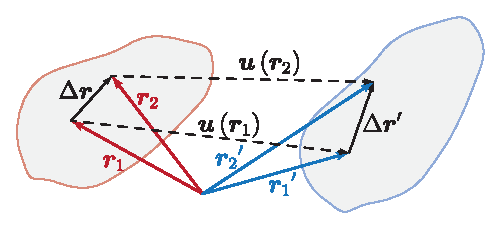
\includegraphics[scale=1]{figs/u.eps}
\caption{Az ${\mathbf{u}}\left( {\mathbf{r}} \right)$ elmozdulásmező szemléltetése.}
\label{fig:u}
\end{figure}
Ekkor az ábráról leolvasható módon
\[\begin{aligned}
  \underbrace {{{\mathbf{r}}_2}' - {{\mathbf{r}}_1}'}_{\Delta {\mathbf{r}}'} =  & {\mathbf{u}}\left( {{{\mathbf{r}}_2}} \right) + \underbrace {{{\mathbf{r}}_2} - {{\mathbf{r}}_1}}_{\Delta {\mathbf{r}}} - {\mathbf{u}}\left( {{{\mathbf{r}}_1}} \right) \\ 
  \Delta {\mathbf{r}}' =  & \Delta {\mathbf{r}} + {\mathbf{u}}\left( {{{\mathbf{r}}_1} + \Delta {\mathbf{r}}} \right) - {\mathbf{u}}\left( {{{\mathbf{r}}_1}} \right), \\ 
\end{aligned} \]
így ha ${\Delta {\mathbf{r}}}$ elég kicsi, akkor írhatjuk ezt úgy, hogy 
\begin{equation} \label{eq:disztrozio_def}
\Delta {\mathbf{r}}' = \Delta {\mathbf{r}} + {\left. {\frac{{d{\mathbf{u}}\left( {\mathbf{r}} \right)}}{{d{\mathbf{r}}}}} \right|_{{{\mathbf{r}}_1}}} \cdot \Delta {\mathbf{r}} = \underbrace {\left( {{\mathbf{I}} + {{\left. {{{\mathbf{\beta }}^T}} \right|}_{{{\mathbf{r}}_1}}}} \right)}_{\mathbf{F}}\Delta {\mathbf{r}},
\end{equation}
ahol a bevezetett ${\mathbf{\beta }}$ a \textbf{disztorzió}, és ezen \eqref{eq:disztrozio_def}.\ képlet szerint a definíciója:
\begin{equation} \label{eq:disztrozio_szamolas}
{\beta _{ij}} = {\partial _i}{u_j} \Leftrightarrow {{\mathbf{\beta }}^T}\left( {\mathbf{r}} \right) = \frac{{d{\mathbf{u}}}}{{d{\mathbf{r}}}},
\end{equation}
valamint bevezethetjük még a \textbf{deformációs gradienst}, amelyre
\[{\mathbf{F}}\left( {\mathbf{r}} \right) = \frac{d}{{d{\mathbf{r}}}}\left( {{\mathbf{r}} + {\mathbf{u}}\left( {\mathbf{r}} \right)} \right) = {\mathbf{I}} + {{\mathbf{\beta }}^T}\left( {\mathbf{r}} \right).\]
\subsection{Deformáció}
Fejezzük ki az anyagban két pont távolságának a megváltozását, azaz $\left| {\Delta {\mathbf{r}}'} \right| - \left| {\Delta {\mathbf{r}}} \right|$ mennyiséget! Ehhez először fejezzük ki ${\left| {\Delta {\mathbf{r}}'} \right|^2}$-et:
\[\begin{aligned}
  {\left| {\Delta {\mathbf{r}}'} \right|^2} =  & \Delta {\mathbf{r}}' \cdot \Delta {\mathbf{r}}' \\ 
   =  & \left( {{\mathbf{I}} + {{\mathbf{\beta }}^T}} \right)\Delta {\mathbf{r}} \cdot \left( {{\mathbf{I}} + {{\mathbf{\beta }}^T}} \right)\Delta {\mathbf{r}} \\ 
   =  & \Delta {\mathbf{r}}\underbrace {\left( {{\mathbf{I}} + {\mathbf{\beta }}} \right)\left( {{\mathbf{I}} + {{\mathbf{\beta }}^T}} \right)}_{\left( {{\mathbf{I}} + {\mathbf{\beta }} + {{\mathbf{\beta }}^T} + {\mathbf{\beta }}{{\mathbf{\beta }}^T}} \right)}\Delta {\mathbf{r}} \\ 
   =  & {\left( {\Delta {\mathbf{r}}} \right)^2} + \Delta {\mathbf{r}}\left( {{\mathbf{\beta }} + {{\mathbf{\beta }}^T} + {\mathbf{\beta }}{{\mathbf{\beta }}^T}} \right)\Delta {\mathbf{r}} .\\ 
\end{aligned} \]
Ebből
\begin{align} \label{eq:deform_def}
  \left| {\Delta {\mathbf{r}}'} \right| =  & \left| {\Delta {\mathbf{r}}} \right|\sqrt {1 + \frac{{\Delta {\mathbf{r}}}}{{\left| {\Delta {\mathbf{r}}} \right|}}\left( {{\mathbf{\beta }} + {{\mathbf{\beta }}^T} + {\mathbf{\beta }}{{\mathbf{\beta }}^T}} \right)\frac{{\Delta {\mathbf{r}}}}{{\left| {\Delta {\mathbf{r}}} \right|}}}  \nonumber \\ 
   =  & \left| {\Delta {\mathbf{r}}} \right|\sqrt {1 + {{\mathbf{e}}_{\Delta {\mathbf{r}}}}2{\mathbf{\varepsilon }}{{\mathbf{e}}_{\Delta {\mathbf{r}}}}},
\end{align}
ahol bevezettük az ${\Delta {\mathbf{r}}}$ irányú egységvektort, ${{\mathbf{e}}_{\Delta {\mathbf{r}}}}$-t, illetve a deformációs tenzort,
\[2{\mathbf{\varepsilon }}\left( {\mathbf{r}} \right) = {\mathbf{\beta }}\left( {\mathbf{r}} \right) + {{\mathbf{\beta }}^T}\left( {\mathbf{r}} \right) + {\mathbf{\beta }}\left( {\mathbf{r}} \right){{\mathbf{\beta }}^T}\left( {\mathbf{r}} \right).\]
Ha a disztorzió kicsi, akkor ${\mathbf{\beta }}\left( {\mathbf{r}} \right){{\mathbf{\beta }}^T}\left( {\mathbf{r}} \right)$ elhanyagolható ${\mathbf{\beta }}\left( {\mathbf{r}} \right)$-hoz képest, és 
\begin{equation}
{\mathbf{\varepsilon }}\left( {\mathbf{r}} \right) = \frac{{{\mathbf{\beta }}\left( {\mathbf{r}} \right) + {{\mathbf{\beta }}^T}\left( {\mathbf{r}} \right)}}{2}.
\end{equation}
Viszont ekkor ${\mathbf{\varepsilon }}$ is kicsi, így \az{\eqref{eq:deform_def}} egyenletben a gyököt 1 körül sorfejtve kapjuk, hogy
\[\left| {\Delta {\mathbf{r}}'} \right| = \left| {\Delta {\mathbf{r}}} \right|\left( {1 + \frac{{{{\mathbf{e}}_{\Delta {\mathbf{r}}}}2{\mathbf{\varepsilon }}{{\mathbf{e}}_{\Delta {\mathbf{r}}}}}}{2}} \right) \Rightarrow \frac{{\left| {\Delta {\mathbf{r}}'} \right|}}{{\left| {\Delta {\mathbf{r}}} \right|}} - 1 = {{\mathbf{e}}_{\Delta {\mathbf{r}}}}{\mathbf{\varepsilon }}{{\mathbf{e}}_{\Delta {\mathbf{r}}}}.\]
Itt megjelent a ${\Delta {\mathbf{r}}}$ (avagy vesszős?) irányú relatív hosszváltozás. Fontos, hogy ez a formula csak akkor igaz, ha a disztorzió kicsi volt. Ez nem csak, hogy egyszerűbb alakra hozta a deformációt a disztorzió függvényeként, de a relatív hosszváltozás is egyszerűbben kifejezhetővé vált.

\subsubsection{Relatív térfogatváltozás}
Nézzük meg, hogyan változik meg egy $V$ nagyságú térfogatelem, amelyet a
\[{\mathbf{x}} = \left( {\begin{array}{*{20}{c}}
  1 \\ 
  0 \\ 
  0 
\end{array}} \right)x,\quad {\mathbf{y}} = \left( {\begin{array}{*{20}{c}}
  0 \\ 
  1 \\ 
  0 
\end{array}} \right)y,\quad {\mathbf{z}} = \left( {\begin{array}{*{20}{c}}
  0 \\ 
  0 \\ 
  1 
\end{array}} \right)z\]
vektorok kijelölnek! Ez könnyedén kifejezhető a három vektor vegyesszorzatával, azaz
\[V = \left( {{\mathbf{x}},{\mathbf{y}},{\mathbf{z}}} \right) = \left| {\begin{array}{*{20}{c}}
  x&0&0 \\ 
  0&y&0 \\ 
  0&0&z 
\end{array}} \right| = x \cdot y \cdot z.\]
Legyenek ezek a vektorok elég kicsik abban az értelemben, hogy ${\mathbf{F}}$ legyen konstans a vektorok által kijelölt térfogatban, ${\mathbf{y}}' = {\mathbf{Fy}}$, ${\mathbf{x}}' = {\mathbf{Fx}}$ és ${\mathbf{z}}' = {\mathbf{Fz}}$. Ekkor a transzformáció után a vektorok alakja:
\[{\mathbf{x}}' = \left( {\begin{array}{*{20}{c}}
  {1 + {\partial _x}{u_x}} \\ 
  {{\partial _x}{u_y}} \\ 
  {{\partial _x}{u_z}} 
\end{array}} \right)x,\quad {\mathbf{y}}' = \left( {\begin{array}{*{20}{c}}
  {{\partial _y}{u_x}} \\ 
  {1 + {\partial _y}{u_y}} \\ 
  {{\partial _y}{u_z}} 
\end{array}} \right)y,\quad {\mathbf{z}}' = \left( {\begin{array}{*{20}{c}}
  {{\partial _z}{u_x}} \\ 
  {{\partial _z}{u_y}} \\ 
  {1 + {\partial _z}{u_z}} 
\end{array}} \right)z,\]
az új térfogatra pedig
\begin{equation*}
  V' = \left( {{\mathbf{x}}',{\mathbf{y}}',{\mathbf{z}}'} \right) = \left| {\begin{array}{*{20}{c}}
  {1 + {\partial _x}{u_x}}&{{\partial _x}{u_y}}&{{\partial _x}{u_z}} \\ 
  {{\partial _y}{u_x}}&{1 + {\partial _y}{u_y}}&{{\partial _y}{u_z}} \\ 
  {{\partial _z}{u_x}}&{{\partial _z}{u_y}}&{1 + {\partial _z}{u_z}} 
\end{array}} \right| x y z  = \det \left( {\mathbf{F}} \right)V. 
\end{equation*}
Az új térfogat a régihez viszonyítva, illetve a relatív térfogatváltozásra kapjuk, hogy
\[\frac{{V'}}{V} = \det \left( {\mathbf{F}} \right) \Leftrightarrow \frac{{V' - V}}{V} = \frac{{\Delta V}}{V} = \det \underbrace {\left( {{\mathbf{I}} + {\mathbf{\beta^T }}} \right)}_{\mathbf{F}} - 1.\]
Gyakori eset, hogy a deriváltak az $1$-hez képest kicsik, így elsőrendig megtartva a determináns tagjait, a másod- és magasabbrendű tagokat pedig elhanyagolva kapjuk, hogy 
\begin{multline*}
  V' \approx \left( {1 + {\partial _x}{u_x}} \right)\left( {1 + {\partial _y}{u_y}} \right)\left( {1 + {\partial _z}{u_z}} \right)V \approx \left( {1 + {\partial _x}{u_x} + {\partial _y}{u_y} + {\partial _z}{u_z}} \right)V =  \\
   = \left( 1+{{\text{Tr}}\left( {\mathbf{\epsilon}} \right)} \right)V,
\end{multline*}
ahol megjelent a deformációs tenzor trace-e, avagy spúrja, amit a ${\text {Tr}}$ vagy ${\text {Sp}}$ operátor jelöl, ami megadja a főátlóbeli elemek összegét. Ekkor a relatív térfogatváltozás egyszerűen a deformációs tenzor trace-e, azaz
\[\frac{{V' - V}}{V} = \frac{{\Delta V}}{V} = {\text{Tr}}\left( {\mathbf{\varepsilon }} \right).\]

\subsubsection{Szimmetrikus, antiszimmetrikus rész}
Vezessük be egy operátor szimmetrikus és nem szimmetrikus részének a definícióját:
\[{{\mathbf{A}}^{{\text{sz}}}} = \frac{{{\mathbf{A}} + {{\mathbf{A}}^T}}}{2}\quad {{\mathbf{A}}^{\text{asz}}} = \frac{{{\mathbf{A}} - {{\mathbf{A}}^T}}}{2},\]
ahol a $T$ index a transzponálást jelenti. Ekkor minden operátor felírható ezek összegeként,
\[{\mathbf{A}} = {{\mathbf{A}}^{{\text{sz}}}} + {{\mathbf{A}}^{{\text{asz}}}},\]
valamint igaz erre a felbontásra, hogy \[{\left( {{{\mathbf{A}}^{{\text{sz}}}}} \right)^T} = {{\mathbf{A}}^{\text{sz}}}\quad {\left( {{{\mathbf{A}}^{{\text{asz}}}}} \right)^T} =  - {{\mathbf{A}}^{{\text{asz}}}}.\]
Ekkor \az{\eqref{eq:disztrozio_def}} egyenletet az alábbi formában írhatjuk:
\[\Delta {\mathbf{r}}' = \left( {{\mathbf{I}} + {{\mathbf{\beta }}^{sz}} + {{\mathbf{\beta }}^{{\text{asz}}}}} \right)\Delta {\mathbf{r}}.\] A terminológia szerint csakis akkor igaz, hogy ${{\mathbf{\beta }}^{sz}} = {\mathbf{\varepsilon }}$ a \textbf{deformációs tenzor}, ha a disztorzió kicsi.

\subsection{Egyszerű transzformációk}
\subsubsection{Eltolás}
Eltolásnál minden régi helyvektorhoz egy ${{\mathbf{r}}_0}$ helyvektort adunk, amelyet \az{\ref{fig:eltolas}}.\ ábra szemléltet. Ekkor
\[{\mathbf{r}}'\left( {\mathbf{r}} \right) = {\mathbf{r}} + {{\mathbf{r}}_0}.\]
\begin{figure}[htb] 
\centering    
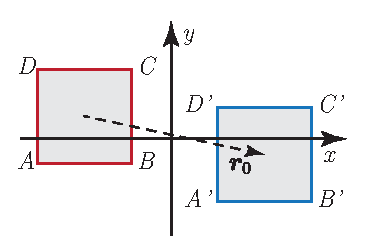
\includegraphics[scale=1]{figs/eltolas.eps}
\caption{Az eltolás szemléltetése.}
\label{fig:eltolas}
\end{figure}
Ekkor az elmozdulástér
\[{\mathbf{u}} = {{\mathbf{r}}_0},\]
a disztorziót pedig vagy számolhatjuk egyből ${\mathbf{u}}$ deriváltjából, vagy leolvashatjuk a $\Delta {\mathbf{r}}'$ értékéből,
\[\Delta {{\mathbf{r}}^\prime } = {{\mathbf{r}}_2}^\prime  - {{\mathbf{r}}_1}^\prime  = \left( {{{\mathbf{r}}_2} + {{\mathbf{r}}_0}} \right) - \left( {{{\mathbf{r}}_1} + {{\mathbf{r}}_0}} \right) = \Delta {\mathbf{r}} = \left( {{\mathbf{I}} + {\mathbf{0}}} \right)\Delta {\mathbf{r}} \Rightarrow \left\{ {\begin{array}{*{20}{c}}
  {{{\mathbf{\beta }}^T} = {\mathbf{0}}} \\ 
  {{\mathbf{F}} = {\mathbf{I}}} 
\end{array}} \right..\]
Triviálisan látszik, hogy a deformáció ${\mathbf{0}}$.

\subsubsection{Nyújtás}
Nyújtásnál minden régi helyvektort (megfelelő koordináta rendszerben) komponensenként egy számmal szorzunk, amelyet \az{\ref{fig:nyujtas}}.\ ábra szemléltet. Ekkor
\begin{multline*}
{\mathbf{r}}'\left( {\mathbf{r}} \right) = \left( {\begin{array}{*{20}{c}}
  {x'} \\ 
  {y'} \\ 
  {z'} 
\end{array}} \right) = \left( {\begin{array}{*{20}{c}}
  {{\lambda _1}x} \\ 
  {{\lambda _2}y} \\ 
  {{\lambda _3}z} 
\end{array}} \right) = \left( {\begin{array}{*{20}{c}}
  {{\lambda _1}}&0&0 \\ 
  0&{{\lambda _2}}&0 \\ 
  0&0&{{\lambda _3}} 
\end{array}} \right)\left( {\begin{array}{*{20}{c}}
  x \\ 
  y \\ 
  z 
\end{array}} \right) = \\ = \left[ {{\lambda _1}\left( {{{\mathbf{e}}_1} \circ {{\mathbf{e}}_1}} \right) + {\lambda _2}\left( {{{\mathbf{e}}_2} \circ {{\mathbf{e}}_2}} \right) + {\lambda _3}\left( {{{\mathbf{e}}_3} \circ {{\mathbf{e}}_3}} \right)} \right]{\mathbf{r}},
\end{multline*}
amelyben ${\lambda _i} \in \mathbb{R}$.

Ekkor az elmozdulástér
\[{\mathbf{u}}\left( {\mathbf{r}} \right) = {\mathbf{r}}' - {\mathbf{r}} = \underbrace {\left( {\begin{array}{*{20}{c}}
  {{\lambda _1}}&0&0 \\ 
  0&{{\lambda _2}}&0 \\ 
  0&0&{{\lambda _3}} 
\end{array}} \right)}_{\mathbf{\lambda }}{\mathbf{r}} - {\mathbf{r}} = \left( {{\mathbf{\lambda }} - {\mathbf{I}}} \right){\mathbf{r}} = \left( {\begin{array}{*{20}{c}}
  {{\lambda _1} - 1}&0&0 \\ 
  0&{{\lambda _2} - 1}&0 \\ 
  0&0&{{\lambda _3} - 1} 
\end{array}} \right){\mathbf{r}},\]
amelyből deriválással megkapható a disztorzió, vagy kifejezhetjük $\Delta {\mathbf{r}}'$-t is,
\[\Delta {\mathbf{r}}' = {{\mathbf{r}}_2}' - {{\mathbf{r}}_1}' = {\mathbf{\lambda }}{{\mathbf{r}}_2} - {\mathbf{\lambda }}{{\mathbf{r}}_1} = {\mathbf{\lambda }}\Delta {\mathbf{r}} = \underbrace {\left( {{\mathbf{I}} + \left( {{\mathbf{\lambda }} - {\mathbf{I}}} \right)} \right)}_{{\mathbf{F}} = {\mathbf{I}} + {{\mathbf{\beta }}^T}}\Delta {\mathbf{r}}\]
amelyből egyszerűen leolvasható a disztorzió transzponáltja és a deformációs gradiens.


Egy speciális eset, ha a  nyújtás iránytól független, azaz izotróp: ${\lambda _1} = {\lambda _2} = {\lambda _3}$, ekkor az ${\mathbf{I}}$ egységoperátorral
\[{\mathbf{r}}'\left( {\mathbf{r}} \right) = {\lambda _1}{\mathbf{r}} = {\lambda _1}{\mathbf{Ir}}.\] Másik speciális eset a tiszta nyírás (lásd \ref{sec:tiszta_nyiras}).
\begin{figure}[htb] 
\centering    
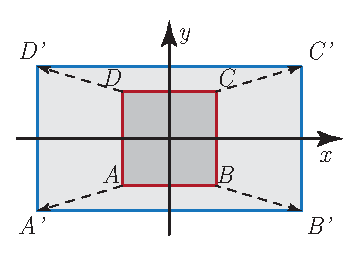
\includegraphics[scale=1]{figs/nyujtas.eps}
\caption{A nyújtás szemléltetése.}
\label{fig:nyujtas}
\end{figure}
\subsubsection{Forgatás}
Forgatásnál minden régi helyvektor nagysága megmarad, csak az irányuk változik meg. A forgatást jellemezzük a szöggel és a forgatás tengelyének az irányával. Egy $z$ tengelyű, $\alpha$ szögű forgatásra
\[{\mathbf{r}}'\left( {\mathbf{r}} \right) = \left( {\begin{array}{*{20}{c}}
  {\cos \left( \alpha  \right)}&{ - \sin \left( \alpha  \right)}&0 \\ 
  { \sin \left( \alpha  \right)}&{\cos \left( \alpha  \right)}&0 \\ 
  0&0&1 
\end{array}} \right)\left( {\begin{array}{*{20}{c}}
  x \\ 
  y \\ 
  z 
\end{array}} \right) = {{\mathbf{O}}_{z,\alpha }}{\mathbf{r}}.\]
Egyezmény szerint a pozitív szögű forgatás óramutató járásával ellentétes irányt jelent, és a mátrixban az első sorban van a negatív előjel. Ezt \az{\ref{fig:eltolas}}.\ ábra szemlélteti. (A $z$ tengely a papír síkjából kifelé jön, így alkotnak a tengelyek jobbsodrású rendszert.) Általánosan számolással megmutatható, hogy akárhány forgatás együttes hatása szintén egyetlen forgatás egy jól megválasztott tengely körül, jól megválasztott szöggel.

\begin{figure}[htb] 
\centering    
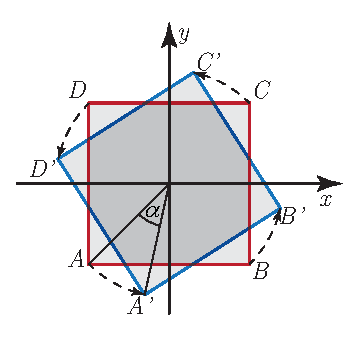
\includegraphics[scale=1]{figs/forgatas.eps}
\caption{A forgatás szemléltetése.}
\label{fig:forgat}
\end{figure}

Az elmozdulástér ekkor:
\[{\mathbf{u}}\left( {\mathbf{r}} \right) = {\mathbf{r}}' - {\mathbf{r}} = {\mathbf{Or}} - {\mathbf{r}} = \left( {{\mathbf{O}} - {\mathbf{I}}} \right){\mathbf{r}}.\]
Ennek deriváltjaként előáll a disztorzió, de megkaphatjuk abból is, ha kiszámoljuk $\Delta {\mathbf{r}}'$-t:
\[\Delta {\mathbf{r}}' = {{\mathbf{r}}_2}' - {{\mathbf{r}}_1}' = {\mathbf{O}}{{\mathbf{r}}_2} - {\mathbf{O}}{{\mathbf{r}}_1} = {\mathbf{O}}\Delta {\mathbf{r}}.\]
Ebből már látható a deformációs gradiensre és a disztorzióra, hogy 
\[{\mathbf{F}} = {\mathbf{O}}\quad {{\mathbf{\beta }}^T} = {\mathbf{O}} - {\mathbf{I}}.\]
\paragraph{Infinitezimális forgatás}
Legyen az elmozdulásmezőnk
\begin{equation} \label{eq:inf_forgat}
{{\mathbf{u}}^f}\left( {\mathbf{r}} \right) = \Delta {\mathbf{\varphi }} \times {\mathbf{r}},
\end{equation}
azaz egy infinitezimális forgatás (azaz $\Delta {\mathbf{\varphi }} = \left( {0,0,\Delta \varphi } \right)$ nagyon kicsi), ahol $\Delta {\mathbf{\varphi }}$ értéke helytől független. A hozzá tartozó disztorzió:
\[\beta _{ij}^f = {\partial _i}{\varepsilon _{jkl}}\Delta {\varphi _k}{x_l} = {\varepsilon _{jkl}}\Delta {\varphi _k}\underbrace {{\partial _i}{x_l}}_{{\delta _{il}}} = {\varepsilon _{jki}}\Delta {\varphi _k} = {\varepsilon _{ijk}}\Delta {\varphi _k}.\]
Vegyük észre, hogy 
\[\beta _{ji}^f = {\varepsilon _{jik}}\Delta {\varphi _k} =  - {\varepsilon _{ijk}}\Delta {\varphi _k} =  - \beta _{ij}^f,\]
vagyis
\[\left\{ {{{\left( {{{\mathbf{\beta }}^f}} \right)}^T} =  - {{\mathbf{\beta }}^f}} \right\} \Leftrightarrow \left\{ {{{\mathbf{\beta }}^{f,asz}} = {{\mathbf{\beta }}^f}} \right\} \Leftrightarrow \left\{ {{{\mathbf{\beta }}^{f,sz}} = 0} \right\}.\]
Azt látjuk tehát, hogy egy homogén elforgatás disztorziója tisztán antiszimmetrikus, így a deformáció egzaktul 0, ha a forgatás kicsi. 

Egy általános, infinitezimális disztorziónak sem a szimmetrikus, sem az antiszimmetrikus része nem 0. De a kettőhöz külön-külön definiálható egy infinitezimális transzformáció, amelyek közül az antiszimmetrikushoz egy tiszta forgatás tartozik.

\paragraph{Véges nagyságú forgatás}
Láthattuk az előző részben, hogy az infinitezimális forgatás deformációja egzaktul 0, hiszen a disztorzió szimmetrikus része 0. Egy véges forgatás előáll apró forgatások összegeként, ezért azt várjuk, hogy véges forgatásra is 0 legyen a deformáció.

\subsection{Feladatok}
Feladatok a feladatlapon.

\subsection{Általános transzformációk}
Végsősoron minden transzformáció előáll helyfüggő eltolási transzformációként, hiszen "csupán" a ${\mathbf{u}}\left( {\mathbf{r}} \right)$ eltolásvektort kell megadni a hely függvényében, ${\mathbf{r}}'\left( {\mathbf{r}} \right) = {\mathbf{r}} + {\mathbf{u}}\left( {\mathbf{r}} \right)$. Gondolhatunk egy forgatásra is úgy, mint egy olyan eltolásra, ami helyről helyre változik. Viszont egy ilyen eltolás deformációs gradiensének vagy deformációjának kiszámolásában feltettük, hogy az eltolás mértéke helyfüggetlen, így ha ki akarnánk ${\mathbf{F}}$-et vagy ${\mathbf{\varepsilon }}$-et számolni, újra el kéne végezni azokat a műveleteket, amiket a forgatásnál kiszámoltunk.

Praktikus tehát a forgatást és nyújtást alapul vennünk, amelyekre már ismerjük ${\mathbf{F}}$-et és ${\mathbf{\varepsilon }}$. Azonban nem minden transzformáció állítható elő ebből a kettőből úgy, hogy azok értéke helytől független legyen.

\subsubsection{Nyírás}
\paragraph{Általános nyírás}
Egy általános nyírást szemléltet \az{\ref{fig:nyiras}}.\ ábra. Ekkor van olyan vonatkoztatási rendszer, amelyben a főátló elemeinek az értéke $1$, és minden egyéb mátrixelem egyetlen elemet kivéve $0$-ák. A deformációs gradiensre példa a
\[{\mathbf{F}} = \left( {\begin{array}{*{20}{c}}
  1&{0,4} \\ 
  0&1 
\end{array}} \right).\]
A definíció értelmében a determináns mindig 1, így a térfogat (vagy $2D$-ban a felület) nem változik meg. A nyírást feloghatjuk úgy is, mint egy $x$ függő eltolás az $y$ irányba, ahol az eltolás mértéke lineáris függ a koordinátától.

Később látni fogjuk, hogy minden transzformáció felírható tiszta nyújtás és forgatás egymásutánjaként. Egy általános nyírás is felírható úgy, mint egy megfelelő tengely körüli nyújtás, majd egy forgatás. (Lásd: \ref{sec:polaris_dekomp}.)


\paragraph{Tiszta nyírás} \label{sec:tiszta_nyiras}
A tiszta nyírás olyan nyújtás, ahol a térfogatváltozás 0, a deformációs gradiens szimmetrikus, tehát a megfelelő koordinátarendszerben a deformációs gradiens diagonális, és ${\lambda _1}{\lambda _2}{\lambda _3} = 1$. Egy tiszta nyírást szemléltet \az{\ref{fig:tiszta_nyiras}}.\ ábra. A deformációs gradiensre példa lehet a 
\[{\mathbf{F}} = {{\mathbf{O}}_{z,45^\circ }}\left( {\begin{array}{*{20}{c}}
  {1,25}&0 \\ 
  0&{0,8} 
\end{array}} \right){{\mathbf{O}}_{z, - 45^\circ }} = \left( {\begin{array}{*{20}{c}}
  {1,025}&{0,225} \\ 
  {0,225}&{1,025} 
\end{array}} \right),\]
amelyben ${\mathbf{F}}$ a rajzolt koordinátarendszerben meghatározott mátrix, de leolvasható a $45^\circ$-os koordináták melletti értéke is. Egy általános nyírás csak egy forgatással együtt írható le tiszta nyújtással, ekkor viszont a nyújtás épp egy tiszta nyírás. (Lásd: \ref{sec:polaris_dekomp}.)

\begin{figure}[htb] 
\begin{subfigure}[b]{0.45\textwidth}
\centering
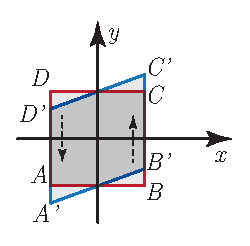
\includegraphics[scale=1]{figs/nyiras.eps}
\caption{A nyírás szemléltetése.}
\label{fig:nyiras}
\end{subfigure} \hfill
\begin{subfigure}[b]{0.45\textwidth}
\centering
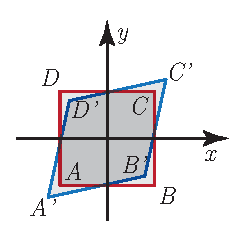
\includegraphics[scale=1]{figs/tiszta_nyiras.eps}
\caption{A tiszta nyírás szemléltetése.}
\label{fig:tiszta_nyiras}
\end{subfigure}
\label{fig_nyujtasok}
\caption{Nyírások szemléltetése.}
\end{figure}


\paragraph{Infinitezimális nyírás}
Infinitezimális nyírások során a ${\mathbf{\beta }}$ vagy ${\mathbf{F}}$ főátlón kívüli nem $0$ elem értékét vesszük infinitezimálisan kicsinek. Általános nyírásnál az ${\mathbf{F}}$ főátlójában eleve $1$-esek voltak, tiszta nyírásnál pedig azért lesznek szintén $1$-esek, mert az $1$-hez képest másodrendben kicsi tagok jelennének csak meg, amit elhanyagolunk. 

\subsection{Feladatok}
Feladatok a feladatlapon.


\subsubsection{Homokóra nyújtás}
Jobb kifejezés hiányában van ez a cím, lehetne még ferdítés. Ekkor a nyújtás mértéke lineárisan függ az egyik tengelytől, és arra merőleges. \Aref{fig:homokora_nyujtas_szamolos}.\ ábra egy ilyet szemléltet (a könnyebb ábrázolásért egy eltolással együtt), ahol a legkisebb $y$ értékű részét a térnek $0{,}75$ szorosára nyújtjuk, a legnagyobb $y$ értékű részt pedig $1{,}25$-szörösére nyújtottuk, a kettő között pedig lineáris az átmenet.
\begin{figure}[htb] 
\centering    
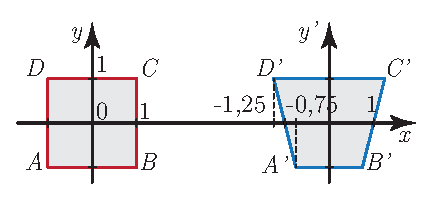
\includegraphics[scale=1]{figs/homokora_nyujtas_szamolos.eps}
\caption{A homokóra nyújtás példájának szemléltetése.}
\label{fig:homokora_nyujtas_szamolos}
\end{figure}

Az elmozdulástérre példa:
\[{\mathbf{u}}\left( {\mathbf{r}} \right) = \frac{1}{4}\left( {\begin{array}{*{20}{c}}
  {x \cdot y} \\ 
  0 
\end{array}} \right).\]
Ekkor a disztorziót deriválással lehet legkönnyebben megkapni,
\[\begin{gathered}
  {\partial _x}{u_x} = y/4 \hfill \\
  {\partial _y}{u_x} = x/4 \hfill \\
  {\partial _x}{u_y} = {\partial _y}{u_y} = 0, \hfill \\ 
\end{gathered} \]
így a disztorzióra és a deformációs gradiensre:
\[{{\mathbf{\beta }}^T} = \left( {\begin{array}{*{20}{c}}
  {y/4}&{x/4} \\ 
  0&0 
\end{array}} \right)\quad {\mathbf{F}} = \left( {\begin{array}{*{20}{c}}
  {1 + y/4}&{x/4} \\ 
  0&1 
\end{array}} \right).\]
\footnotesize
Mi lenne, ha megint a $\Delta {\mathbf{r}}'$-ből szeretnénk számolni a disztorziót és a deformációs gradienst?
\[\Delta {\mathbf{r}}' = {{\mathbf{r}}_2}' - {{\mathbf{r}}_1}' = \left( {{{\mathbf{r}}_2} + {\mathbf{u}}\left( {{{\mathbf{r}}_2}} \right)} \right) - \left( {{{\mathbf{r}}_1} + {\mathbf{u}}\left( {{{\mathbf{r}}_1}} \right)} \right) = \Delta {\mathbf{r}} + {\mathbf{u}}\left( {{{\mathbf{r}}_2}} \right) - {\mathbf{u}}\left( {{{\mathbf{r}}_1}} \right)\]
Most nem tudunk továbblépni, mert ${\mathbf{u}}\left( {\mathbf{r}} \right)$ nem lineáris, azaz ${\mathbf{u}}\left( {\lambda {\mathbf{r}}} \right) \ne \lambda {\mathbf{u}}\left( {\mathbf{r}} \right)$. Továbbhaladni csak akkor tudunk, ha elvégezzük a $\Delta {\mathbf{r}}' \to 0$ limeszt, hogy lehessen aszerint osztani, pontosabban szólva deriválni:
\[d{\mathbf{r}}' = d{\mathbf{r}} + \frac{{{\mathbf{u}}\left( {{{\mathbf{r}}_2}} \right) - {\mathbf{u}}\left( {{{\mathbf{r}}_1}} \right)}}{{d{\mathbf{r}}}} = \left( {{\mathbf{I}} + \frac{{d{\mathbf{u}}\left( {\mathbf{r}} \right)}}{{d{\mathbf{r}}}}} \right)d{\mathbf{r}},\]
vagyis ezúttal is deriváláson keresztül tudunk csak számolni.
\normalsize

Nézzük meg, hogyan hat ez a transzformáció! Vegyünk egy négyzetet, amelynek a sarkainak a koordinátái legyenek 
\[{{\mathbf{r}}_A} = \left( {\begin{array}{*{20}{c}}
  { - 1} \\ 
  { - 1} 
\end{array}} \right)\quad {{\mathbf{r}}_B} = \left( {\begin{array}{*{20}{c}}
  1 \\ 
  { - 1} 
\end{array}} \right)\quad {{\mathbf{r}}_C} = \left( {\begin{array}{*{20}{c}}
  1 \\ 
  1 
\end{array}} \right)\quad {{\mathbf{r}}_D} = \left( {\begin{array}{*{20}{c}}
  { - 1} \\ 
  1 
\end{array}} \right).\]
Ekkor a transzformáció után a sarkok új koordinátáit az elmozdulástérből számolva:
\begin{alignat*}{2}
   & {\mathbf{u}}\left( {{{\mathbf{r}}_A}} \right) = {\mathbf{u}}\left( {\begin{array}{*{20}{c}}
  { - 1} \\ 
  { - 1} 
\end{array}} \right) = \frac{1}{4}\left( {\begin{array}{*{20}{c}}
  1 \\ 
  0 
\end{array}} \right)\quad  && {{\mathbf{r}}_A}' = \left( {\begin{array}{*{20}{c}}
  { - 1} \\ 
  { - 1} 
\end{array}} \right) + \frac{1}{4}\left( {\begin{array}{*{20}{c}}
  1 \\ 
  0 
\end{array}} \right) = \left( {\begin{array}{*{20}{c}}
  { - 0,75} \\ 
  { - 1} 
\end{array}} \right), \\ 
   & {\mathbf{u}}\left( {{{\mathbf{r}}_B}} \right) = {\mathbf{u}}\left( {\begin{array}{*{20}{c}}
  1 \\ 
  { - 1} 
\end{array}} \right) = \frac{1}{4}\left( {\begin{array}{*{20}{c}}
  { - 1} \\ 
  0 
\end{array}} \right)\quad  && {{\mathbf{r}}_B}' = \left( {\begin{array}{*{20}{c}}
  1 \\ 
  { - 1} 
\end{array}} \right) + \frac{1}{4}\left( {\begin{array}{*{20}{c}}
  { - 1} \\ 
  0 
\end{array}} \right) = \left( {\begin{array}{*{20}{c}}
  {0,75} \\ 
  { - 1} 
\end{array}} \right), \\ 
   & {\mathbf{u}}\left( {{{\mathbf{r}}_C}} \right) = {\mathbf{u}}\left( {\begin{array}{*{20}{c}}
  1 \\ 
  1 
\end{array}} \right) = \frac{1}{4}\left( {\begin{array}{*{20}{c}}
  1 \\ 
  0 
\end{array}} \right)\quad  && {{\mathbf{r}}_C}' = \left( {\begin{array}{*{20}{c}}
  1 \\ 
  1 
\end{array}} \right) + \frac{1}{4}\left( {\begin{array}{*{20}{c}}
  1 \\ 
  0 
\end{array}} \right) = \left( {\begin{array}{*{20}{c}}
  {1,25} \\ 
  { 1} 
\end{array}} \right), \\ 
   & {\mathbf{u}}\left( {{{\mathbf{r}}_D}} \right) = {\mathbf{u}}\left( {\begin{array}{*{20}{c}}
  { - 1} \\ 
  1 
\end{array}} \right) = \frac{1}{4}\left( {\begin{array}{*{20}{c}}
  { - 1} \\ 
  0 
\end{array}} \right)\quad  && {{\mathbf{r}}_D}' = \left( {\begin{array}{*{20}{c}}
  { - 1} \\ 
  1 
\end{array}} \right) + \frac{1}{4}\left( {\begin{array}{*{20}{c}}
  { - 1} \\ 
  0 
\end{array}} \right) = \left( {\begin{array}{*{20}{c}}
  { - 1,25} \\ 
  { 1} 
\end{array}} \right).
\end{alignat*}
Ezeket az értékeket nem kaphattuk volna meg abból, hogyha megadjuk az ${\mathbf{F}}$ vagy a ${\mathbf{\beta }}$ értékeit a négy sarokban, mert ezek az operátorok az adott helyben definiált $\Delta {\mathbf{r}}$ vektorra hatnak. A deformációs gradiens értékei az egyes sarkokban:
\[{{\mathbf{F}}_A} = \frac{1}{4}\left( {\begin{array}{*{20}{c}}
  3&{ - 1} \\ 
  0&4 
\end{array}} \right)\quad {{\mathbf{F}}_B} = \frac{1}{4}\left( {\begin{array}{*{20}{c}}
  3&1 \\ 
  0&4 
\end{array}} \right)\quad {{\mathbf{F}}_C} = \frac{1}{4}\left( {\begin{array}{*{20}{c}}
  5&1 \\ 
  0&4 
\end{array}} \right)\quad {{\mathbf{F}}_D} = \frac{1}{4}\left( {\begin{array}{*{20}{c}}
  5&{ - 1} \\ 
  0&4 
\end{array}} \right),\]
illetve
\[{\mathbf{\beta }}_A^T = \frac{1}{4}\left( {\begin{array}{*{20}{c}}
  { - 1}&{ - 1} \\ 
  0&0 
\end{array}} \right)\quad {\mathbf{\beta }}_B^T = \frac{1}{4}\left( {\begin{array}{*{20}{c}}
  { - 1}&1 \\ 
  0&0 
\end{array}} \right)\quad {\mathbf{\beta }}_C^T = \frac{1}{4}\left( {\begin{array}{*{20}{c}}
  1&1 \\ 
  0&0 
\end{array}} \right)\quad {\mathbf{\beta }}_D^T = \frac{1}{4}\left( {\begin{array}{*{20}{c}}
  1&{ - 1} \\ 
  0&0 
\end{array}} \right),\]
a négyzet közepén viszont \[{{\mathbf{F}}_0} = {\mathbf{I}}\quad {\mathbf{\beta_0 }} = 0,\]
így itt nincs deformáció. Ha veszek egy olyan $\Delta {\mathbf{r}}$ vektort, ami az origóból indul és a négyzet sarkára mutat, akkor a különböző részein különböző volna a deformáció.


\subsubsection{Csavarás}
A csavarás $3D$-ban értelmezhető transzformáció, amelynek során egy tengely mentén ugyanazon tengely irányában forgatunk, és a forgatás mértéke az anyag tengely menti két vége között folytonosan változik, legegyszerűbb esetben lineárisan.

Képzeljünk el egy $z$ tengelyű négyzetes hasábot, amely $z$-ben $-z_0$-tól $z_0$-ig terjed. Ekkor ennek minden $z$ síkbeli keresztmetszete négyzet. Forgassuk el a $-z_0$-ban lévő részét $z$ tengely mentén $-\alpha$ szöggel, azaz arra a síklapra alkalmazzunk egy ${{\mathbf{O}}_{z, - \alpha }}$ transzformációt. A $z_0$-ban lévő részét szintén $z$ tengely körül, de $\alpha$ szöggel. $-z_0$ és $z_0$ között pedig minden további keresztmetszetében lineárisan változzon a szög $-\alpha$ és $\alpha$ között, azaz pl.\ a $z^*$ keresztmetszeten egy 
\begin{equation}
\left( {\begin{array}{*{20}{c}}
  x \\ 
  y \\ 
  {{z^ * }} 
\end{array}} \right)' = {{\mathbf{O}}_{z,\alpha  \cdot {z^ * }/z_0}} \left( {\begin{array}{*{20}{c}}
  x \\ 
  y \\ 
  {{z^ * }} 
\end{array}} \right)
\end{equation}
forgatást hajtunk végre.

\subsubsection{Lineárisan interpolált transzformációk}
Még megannyi más deformáció fajta is elképzelhető. Volna lehetőség arra, hogy megadjuk például, hogy a transzformáció mibe viszi át az egységnégyzetet. Ekkor megnézhetjük, hogy az egyes oldalakat mennyire nyújtotta meg a deformáció, majd minden pontra lineáris interpolációval meghatározhatnánk az abban a pontban érvényes elmozdulás értékét.

\begin{figure}[htb] 
\centering    
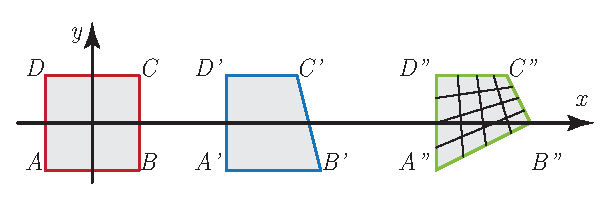
\includegraphics[scale=1]{figs/linearisan_interpolalt.eps}
\caption{Az elmozdulásmezőt lineárisan interpolálhatjuk az oldalélek között.}
\label{fig:linearis_interpolacios_traf}
\end{figure}

\subsection{Feladatok}
Feladatok a feladatlapon.

\subsection{Transzformációk egymásutánja}
Ha alkalmazunk egy transzformációt a mintán, majd az így kapotton újra, akkor az egyes transzformációhoz deformációs gradienst (ill.\ a transzponáltjaikat) össze kell szorozni \az{\eqref{eq:disztrozio_def}} egyenlet szerint, hogy megkapjuk $\Delta {\mathbf{r}}''$-t:
\[1 + {{\mathbf{\beta }}_{AB}} = \left( {1 + {{\mathbf{\beta }}_A}} \right)\left( {1 + {{\mathbf{\beta }}_B}} \right) = \left( {1 + {{\mathbf{\beta }}_A} + {{\mathbf{\beta }}_B} + {{\mathbf{\beta }}_A}{{\mathbf{\beta }}_B}} \right) \ne 1 + {{\mathbf{\beta }}_{BA}}.\]
Láthatjuk, hogy ez nem kommutatív, a transzformációk egymással nem felcserélhetők. Azonban ha a disztorzió elég kicsi, és így a szorzatuk elhanyagolható, akkor már kummutatív, ugyanis 
\begin{equation} \label{eq:deform_kommutatív}
1 + {{\mathbf{\beta }}_{AB}} = \left( {1 + {{\mathbf{\beta }}_A}} \right)\left( {1 + {{\mathbf{\beta }}_B}} \right) = \left( {1 + {{\mathbf{\beta }}_A} + {{\mathbf{\beta }}_B}\underbrace { + {{\mathbf{\beta }}_A}{{\mathbf{\beta }}_B}}_{ \approx 0}} \right) = 1 + {{\mathbf{\beta }}_A} + {{\mathbf{\beta }}_B} = 1 + {{\mathbf{\beta }}_{BA}}.
\end{equation}
(Mit jelent ez a deformációs gradiensre és a deformációra nézve?)

Egy forgatás nem hoz létre deformációt. Ha a transzformáció nem tisztán forgatást ír le, akkor a tisztán forgatást leíró része nem hoz létre deformációt, csak a maradék. Mi az, hogy része? Hogyan hattathatóak a transzformációk egymás után, és hogyan olvasható le, hogy mekkora az eredő deformáció?

\subsubsection{Poláris dekompozíció} \label{sec:polaris_dekomp}
\Az{\eqref{eq:disztrozio_def}} egyenletből láthatóan az ${\mathbf{F}} = 1 + {{\mathbf{\beta }}^T}$ mennyiségek összeszorzódnak. Jelöljön ${\mathbf{O}}$ egy ortogonális mátrixot (ilyenek voltak a forgatás mátrix transzformációs mátrixai), ${\mathbf{U}}$ pedig egy szimmetrikus mátrxiot (ilyenek voltak a tiszta nyújtás mátrixai)! Megmutatjuk, hogyha ${\mathbf{F}}$ invertálható, akkor (egyértelműen) felírható ${\mathbf{F}} = {\mathbf{OU}}$ alakban!
Legyen
\[{{\mathbf{F}}^T}{\mathbf{F}} = {\mathbf{VD}}{{\mathbf{V}}^T},\]
ahol ${\mathbf{V}}$ ortogonális, ${{\mathbf{D}}}$ pedig diagonális mátrix\footnote{Egy diagonális mátrixon értelmezett függvény az egyes mátrxikomponensek ugyanazon függvénye.} Ezt megtehetjük, hisz ${{\mathbf{F}}^T}{\mathbf{F}}$ szimmetrikus, mi több, pozitív definit, így nem csak diagonalizálható, de abból gyököt is vonhatunk, és az inverzét is vehetjük. Ekkor már felbonthatjuk a deformációs gradienst
\[{\mathbf{F}} = \underbrace {{\mathbf{F}}{{\left( {{{\mathbf{F}}^T}{\mathbf{F}}} \right)}^{ - 1/2}}}_{\mathbf{O}}\underbrace {{{\left( {{{\mathbf{F}}^T}{\mathbf{F}}} \right)}^{1/2}}}_{\mathbf{U}}\]
alakban, ahol most belátjuk, hogy ${\mathbf{U}}$ szimmetrikus, illetve, hogy ${\mathbf{O}}$ ortogonális.
Vegyük észre először, hogy 
\[\begin{aligned}
  {\mathbf{V}}\overbrace {{{\mathbf{D}}^{1/2}}\underbrace {{{\mathbf{V}}^T} \cdot {\mathbf{V}}}_{\mathbf{I}}{{\mathbf{D}}^{1/2}}}^{\mathbf{D}}{{\mathbf{V}}^T} = {\mathbf{VD}}{{\mathbf{V}}^T} = {{\mathbf{F}}^T}{\mathbf{F}} \Rightarrow  & {\left( {{{\mathbf{F}}^T}{\mathbf{F}}} \right)^{1/2}} = {\mathbf{V}}{{\mathbf{D}}^{1/2}}{{\mathbf{V}}^T} \\ 
  {\mathbf{V}}\overbrace {{{\mathbf{D}}^{ - 1/2}}\underbrace {{{\mathbf{V}}^T} \cdot {\mathbf{V}}}_{\mathbf{I}}{{\mathbf{D}}^{1/2}}}^{\mathbf{I}}{{\mathbf{V}}^T} = {\mathbf{V}}{{\mathbf{V}}^T} = {\mathbf{I}} \Rightarrow  & {\left( {{{\mathbf{F}}^T}{\mathbf{F}}} \right)^{ - 1/2}} = {\mathbf{V}}{{\mathbf{D}}^{ - 1/2}}{{\mathbf{V}}^T}. \\ 
\end{aligned} \]
Ebből már látszik, hogy 
\[{{\mathbf{U}}^T} = {\left( {{\mathbf{V}}{{\mathbf{D}}^{1/2}}{{\mathbf{V}}^T}} \right)^T} = {\left( {{{\mathbf{V}}^T}} \right)^T}{\left( {{{\mathbf{D}}^{1/2}}} \right)^T}{{\mathbf{V}}^T} = {\mathbf{V}}{{\mathbf{D}}^{1/2}}{{\mathbf{V}}^T} = {{\mathbf{U}}},\]
azaz ${\mathbf{U}} = {{\mathbf{U}}^T}$, tehát ${\mathbf{U}}$ szimmetrikus. Másrészt pedig
\begin{multline*}
{\left( {{\mathbf{F}}{{\left( {{{\mathbf{F}}^T}{\mathbf{F}}} \right)}^{ - 1/2}}} \right)^T} \cdot {\mathbf{F}}{\left( {{{\mathbf{F}}^T}{\mathbf{F}}} \right)^{ - 1/2}} = {\left( {{\mathbf{V}}{{\mathbf{D}}^{ - 1/2}}{{\mathbf{V}}^T}} \right)^T}\underbrace {{{\mathbf{F}}^T} \cdot {\mathbf{F}}}_{{\mathbf{VD}}{{\mathbf{V}}^T}}{\mathbf{V}}{{\mathbf{D}}^{ - 1/2}}{{\mathbf{V}}^T} = \\ = {\mathbf{V}}\overbrace {{{\mathbf{D}}^{ - 1/2}}\underbrace {{{\mathbf{V}}^T}{\mathbf{V}}}_{\mathbf{I}}{\mathbf{D}}\underbrace {{{\mathbf{V}}^T}{\mathbf{V}}}_{\mathbf{I}}{{\mathbf{D}}^{ - 1/2}}}^{\mathbf{I}}{{\mathbf{V}}^T} = {\mathbf{V}}{{\mathbf{V}}^T} = {\mathbf{I}},
\end{multline*}
tehát ${{\mathbf{O}}^T}{\mathbf{O}} = {\mathbf{I}}$, azaz ${\mathbf{O}}$ ortogonális.

Hogyan kaphatjuk tehát meg egy általános ${\mathbf{F}}$-ből, hogy milyen nyújtást és forgatást ír le? A lépések:
\begin{enumerate}
\item ${{{\mathbf{F}}^T}{\mathbf{F}}}$ kiszámolása.
\item Az így kapott szimmetrikus mátrix diagonalizálása egy ${\mathbf{V}}$ és ${\mathbf{V^T}}$ mátrixokkal, ekkor megkapjuk ${\mathbf{D}}$-t.
\item A diagonális mátrix gyökének és az inverzének a gyökének a kiszámítása ${{\mathbf{D}}^{1/2}}$ és ${{\mathbf{D}}^{ - 1/2}}$-hez. Ezt megtehetjük elemenként.
\item Visszaforgatjuk ezeket a mátrixokat az eredeti vonatkoztatási rendszerbe, 
\[\begin{aligned}
  {\mathbf{U}} &  = {\mathbf{V}}{{\mathbf{D}}^{1/2}}{{\mathbf{V}}^T} \\ 
  {\mathbf{O}} &  = {\mathbf{F}} \cdot {\mathbf{V}}{{\mathbf{D}}^{ - 1/2}}{{\mathbf{V}}^T}. \\ 
\end{aligned} \]
\end{enumerate}

\subsubsection{A nemkommutativitás szemléltetése}
Felmerülhet a kérdés, hogy miért épp ${\mathbf{F}} = {\mathbf{OU}}$ alakban bontottuk fel egy általános trasznformációt és miért nem ${\mathbf{F}} = {\mathbf{UO}}$ alakban. Egyáltalán lehetséges egy ilyen felbontás is? És ha igen, mi a különbség?

Még általánosabban felmerülhet a kérdés, hogy mi a szerepe a transzformációk sorrendjének. Nem mindegy, hogy először nyújtom, aztán forgatom, vagy először forgatom, aztán nyújtom?

\paragraph{Példa}
Tekintsük az $x$ irányban kétszeresre nyújtó ${{\mathbf{U}}_2}$, és $z$ tengely kürül $30^\circ$-kal forgató ${{\mathbf{O}}_{z,30^\circ }}$ transzformációt leíró deformációs gradienseket! Ha először nyújtok, aztán forgatok, akkor az eredő deformációs gradiens
\[\begin{aligned}
  {{\mathbf{F}}_{2{\text{ majd }}z,30^\circ }} &  = {{\mathbf{O}}_{z,30^\circ }}{{\mathbf{U}}_2} =  {{\mathbf{F}}_{{\mathbf{OU}}}} = \left( {\begin{array}{*{20}{c}}
  {\cos \left( {30^\circ } \right)}&{ - \sin \left( {30^\circ } \right)} \\ 
  {\sin \left( {30^\circ } \right)}&{\cos \left( {30^\circ } \right)} 
\end{array}} \right)\left( {\begin{array}{*{20}{c}}
  2&0 \\ 
  0&1 
\end{array}} \right) \\ 
   &  = \left( {\begin{array}{*{20}{c}}
  {2\cos \left( {30^\circ } \right)}&{ - \sin \left( {30^\circ } \right)} \\ 
  {2\sin \left( {30^\circ } \right)}&{\cos \left( {30^\circ } \right)} 
\end{array}} \right). \\ 
\end{aligned} \]

Ezzel szenmben, ha először forgatok, aztán nyújtok:
\[\begin{aligned}
  {{\mathbf{F}}_{z,30^\circ {\text{ majd 2}}}} &  = {{\mathbf{U}}_2}{{\mathbf{O}}_{z,30^\circ }} = {{\mathbf{F}}_{{\mathbf{UO}}}} = \left( {\begin{array}{*{20}{c}}
  2&0 \\ 
  0&1 
\end{array}} \right)\left( {\begin{array}{*{20}{c}}
  {\cos \left( {30^\circ } \right)}&{ - \sin \left( {30^\circ } \right)} \\ 
  {\sin \left( {30^\circ } \right)}&{\cos \left( {30^\circ } \right)} 
\end{array}} \right) \\ 
   &  = \left( {\begin{array}{*{20}{c}}
  {2\cos \left( {30^\circ } \right)}&{ - 2\sin \left( {30^\circ } \right)} \\ 
  {\sin \left( {30^\circ } \right)}&{\cos \left( {30^\circ } \right)} 
\end{array}} \right). \\ 
\end{aligned} \]
Láthatjuk, hogy a két deformációs gradiens nem egyezik meg. Nézzük meg, hogy mibe viszi át az egyik, illetve másik transzformáció az  origóra tett négyzetet (legalábbis a jobb felső sarkát)! Ehhez először találjuk ki az elmozdulásmezőt az ${\mathbf{F}} = {\mathbf{I}} + \frac{{d{\mathbf{u}}}}{{d{\mathbf{r}}}}$ összefüggésből:
 \[\begin{gathered}
  {{\mathbf{u}}_{{\mathbf{OU}}}} = \left( {\begin{array}{*{20}{c}}
  {2\cos \left( {30^\circ } \right) - 1}&{ - \sin \left( {30^\circ } \right)} \\ 
  {2\sin \left( {30^\circ } \right)}&{\cos \left( {30^\circ } \right) - 1} 
\end{array}} \right)\left( {\begin{array}{*{20}{c}}
  x \\ 
  y 
\end{array}} \right), \hfill \\
  {{\mathbf{u}}_{{\mathbf{UO}}}} = \left( {\begin{array}{*{20}{c}}
  {2\cos \left( {30^\circ } \right) - 1}&{ - 2\sin \left( {30^\circ } \right)} \\ 
  {\sin \left( {30^\circ } \right)}&{\cos \left( {30^\circ } \right) - 1} 
\end{array}} \right)\left( {\begin{array}{*{20}{c}}
  x \\ 
  y 
\end{array}} \right). \hfill \\ 
\end{gathered} \]
A négyzet új sarka:
\[\begin{aligned}
  \left( {\begin{array}{*{20}{c}}
  1 \\ 
  1 
\end{array}} \right)' &  = \left( {\begin{array}{*{20}{c}}
  1 \\ 
  1 
\end{array}} \right) + {{\mathbf{u}}_{{\mathbf{OU}}}}\left( {\begin{array}{*{20}{c}}
  1 \\ 
  1 
\end{array}} \right) \\ 
   &  = \left( {{{\mathbf{u}}_{{\mathbf{OU}}}} + {\mathbf{I}}} \right)\left( {\begin{array}{*{20}{c}}
  1 \\ 
  1 
\end{array}} \right) \\ 
   &  = \left( {\begin{array}{*{20}{c}}
  {2\cos \left( {30^\circ } \right)}&{ - \sin \left( {30^\circ } \right)} \\ 
  {2\sin \left( {30^\circ } \right)}&{\cos \left( {30^\circ } \right)} 
\end{array}} \right)\left( {\begin{array}{*{20}{c}}
  1 \\ 
  1 
\end{array}} \right) = \left( {\begin{array}{*{20}{c}}
  {2\cos \left( {30^\circ } \right) - \sin \left( {30^\circ } \right)} \\ 
  {2\sin \left( {30^\circ } \right) + \cos \left( {30^\circ } \right)} 
\end{array}} \right). \\ 
\end{aligned} \]
Talán nem meglepő, hogy
\[\underbrace {\left( {\begin{array}{*{20}{c}}
  {\cos \left( {30^\circ } \right)}&{ - \sin \left( {30^\circ } \right)} \\ 
  {\sin \left( {30^\circ } \right)}&{\cos \left( {30^\circ } \right)} 
\end{array}} \right)}_{{{\mathbf{O}}_{z,30^\circ }}}\left( {\begin{array}{*{20}{c}}
  2 \\ 
  1 
\end{array}} \right) = \left( {\begin{array}{*{20}{c}}
  {2\cos \left( {30^\circ } \right) - \sin \left( {30^\circ } \right)} \\ 
  {2\sin \left( {30^\circ } \right) + \cos \left( {30^\circ } \right)} 
\end{array}} \right) = \left( {\begin{array}{*{20}{c}}
  1 \\ 
  1 
\end{array}} \right)',\]
vagyis azt kaptuk, az eredő transzformáció olyan, mintha a már megnyújtott teret elforgattuk volna.

Ha a transzformációkatt felcserélem, akkor
\[\begin{aligned}
  \left( {\begin{array}{*{20}{c}}
  1 \\ 
  1 
\end{array}} \right)' &  = \left( {\begin{array}{*{20}{c}}
  1 \\ 
  1 
\end{array}} \right) + {{\mathbf{u}}_{{\mathbf{UO}}}}\left( {\begin{array}{*{20}{c}}
  1 \\ 
  1 
\end{array}} \right) \\ 
   &  = \left( {{{\mathbf{u}}_{{\mathbf{UO}}}} + {\mathbf{I}}} \right)\left( {\begin{array}{*{20}{c}}
  1 \\ 
  1 
\end{array}} \right) \\ 
   &  = \left( {\begin{array}{*{20}{c}}
  {2\cos \left( {30^\circ } \right)}&{ - 2\sin \left( {30^\circ } \right)} \\ 
  {\sin \left( {30^\circ } \right)}&{\cos \left( {30^\circ } \right)} 
\end{array}} \right)\left( {\begin{array}{*{20}{c}}
  1 \\ 
  1 
\end{array}} \right) = \left( {\begin{array}{*{20}{c}}
  {2\cos \left( {30^\circ } \right) - 2\sin \left( {30^\circ } \right)} \\ 
  {\sin \left( {30^\circ } \right) + \cos \left( {30^\circ } \right)} 
\end{array}} \right), \\ 
\end{aligned} \]
amelyre pedig az igaz, hogy 
\[\left( {\begin{array}{*{20}{c}}
  2&0 \\ 
  0&1 
\end{array}} \right)\left( {\begin{array}{*{20}{c}}
  {\cos \left( {30^\circ } \right) - \sin \left( {30^\circ } \right)} \\ 
  {\sin \left( {30^\circ } \right) + \cos \left( {30^\circ } \right)} 
\end{array}} \right) = \left( {\begin{array}{*{20}{c}}
  {2\cos \left( {30^\circ } \right) - 2\sin \left( {30^\circ } \right)} \\ 
  {\sin \left( {30^\circ } \right) + \cos \left( {30^\circ } \right)} 
\end{array}} \right) = \left( {\begin{array}{*{20}{c}}
  1 \\ 
  1 
\end{array}} \right)',\]
vagyis azt kaptuk, hogy egy eleve elforgatott teret nyújtottunk meg. A nyújtás iránya azonban nem a négyzet oldalainak irányába mutat. Ez egészen pontosan azt jelenti, hogy abban a vonatkoztatási rendszerben, amelyben a négyzet oldalainak az iránya határozzák meg a vonatkoztatási rendszert, a nyújtási mátrix nem diagonális. A kétfajta transzformációt szemlélteti \aref{fig:nem_kommutativ}.\ ábra.

\begin{figure}[htb] 
\centering    
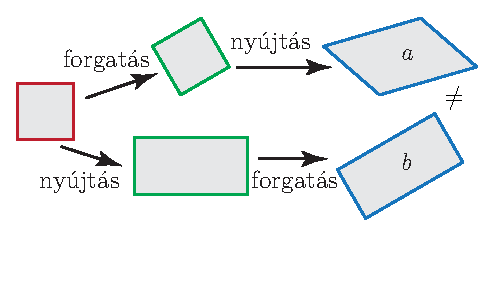
\includegraphics[scale=1]{figs/nem_kommutativ.eps}
\caption[Nem kommutatív transzformációk]{A transzformációk nem felcserélhetőségének illusztációja. A forgatást és nyújtást megadó mátrixok az eredeti vonatkoztatási rendszerben vannak megadva, azonban a testet a 2.\ transzformáció előtt már transzformáltuk egyszer, ellenben a koordinátarendszer nem változott.}
\label{fig:nem_kommutativ}
\end{figure}

Talán azért szokták először a nyújtás, majd a forgatást elvégezni, mert így az alakzat emberek számára könnyebben felismerhető. Ha pedig felismerhető, azért szokták nyújtás, forgatás sorrendben megadni, mert az egyes transzformációk könnyebben leolvashatóak. \Aref{fig:nem_kommutativ}.\ ábra \textit{b} esetét előállíthatnánk egy forgatás és egy tiszta nyírás (amihez szintén egy ortogonális deformációs gradiens tartozik) egymásutánjaként, de ekkor a nyírás elemei nehezebben leolvashatók, az csak a $30^\circ$-os koordinátarendszerben diagonális.

\subsection{Feladatok}
Feladatok a feladatlapon.

\end{document}